\documentclass[conference]{IEEEtran}
\usepackage[T1]{fontenc}
\usepackage{amsmath,amssymb,booktabs,tabularx,array,enumitem}
\usepackage{xcolor,graphicx,tikz,microtype}
\usetikzlibrary{arrows.meta,positioning,fit,backgrounds}
\usepackage{cite,url}
\usepackage[hidelinks]{hyperref}
\definecolor{navy}{HTML}{15354A}
\definecolor{teal}{HTML}{137C80}
\definecolor{pale}{HTML}{EAF4F4}
\hypersetup{pdftitle={Physics-Guided Atom-Wise Attention for Memory-Enhanced Evolutionary RIS Control}}
\setlength{\emergencystretch}{2em}
\setlist{nosep,leftmargin=*}
\renewcommand{\arraystretch}{1.12}
\newcolumntype{Y}{>{\raggedright\arraybackslash}X}
\newcommand{\bvec}{\mathbf b}
\title{Physics-Guided Atom-Wise Attention for Memory-Enhanced Evolutionary RIS Control}
\author{\IEEEauthorblockN{Research Proposal}
\IEEEauthorblockA{Simulation-based study; planned duration: 9--12 months\\Revised 21 October 2026}}
\begin{document}
\raggedbottom
\maketitle
\begin{abstract}
Reconfigurable intelligent surfaces (RISs) control radio propagation through discrete electrical states of many small reflecting elements. Nonideal state responses and changing channels make the reuse of previous configurations imperfect. Memory-enhanced evolutionary control, electromagnetic-aware optimization, and learned genetic operators already exist; their combination alone is therefore insufficient as a novelty claim. This study asks whether a compact, physically conditioned mutation policy can improve the adaptation of remembered RIS configurations under equal online computation budgets. The proposed controller combines an analytical estimate of each bit flip's effect with a learned residual score and conditional selection of a small set of edits. It preserves a shared evolutionary memory and evaluates completed candidates using the same communication--electromagnetic model as every baseline. The principal benchmark uses a 64-element binary RIS, fixed base-station precoding, and two to four users; a single-user case is retained as a diagnostic control because its independent-element structure admits particularly efficient analytical optimization. DeepMIMO-compatible propagation data will be combined with separately validated electromagnetic response tables. Neighbor-dependent coupling will be claimed only where a coupled model has passed independent validation. The evaluation will isolate physical descriptors, attention, conditional edits, and memory; measure wall-clock latency as well as evaluator calls; and test held-out trajectories and physical-response conditions. The intended contribution is evidence about when learning the search operator adds value beyond analytical local search and memory reuse. Fabrication, over-the-air validation, and microcontroller deployment are outside the study's scope.
\end{abstract}
\begin{IEEEkeywords}
Reconfigurable intelligent surface, meta-atom response, learned mutation, attention, evolutionary memory, electromagnetic simulation.
\end{IEEEkeywords}
\section{Motivation and research problem}
An RIS meta-atom is an engineered electromagnetic element, not an atomic particle. Its control bit selects one of two electrical states; those states need not produce equal reflection magnitudes or exactly opposite phases. A metasurface is the array formed by these elements. This project optimizes the electrical state pattern of a fixed array, rather than designing new metal geometries.

A binary array with $N=64$ has $2^{64}$ configurations. That count alone does \emph{not} establish that neural or evolutionary optimization is necessary. Efficient optimal methods exist for the ideal single-user binary beamforming problem \cite{zhang}. Even with nonideal but independent two-state responses, the scalar channel retains strong algebraic structure. A credible proposal must establish where learned search adds value beyond exploiting that structure.

The practical setting is repeated reconfiguration. A useful pattern from a previous channel snapshot may remain a good starting point, but different users, interference, and hardware responses can change which edits are beneficial. Searching combinations of edits can cost more than scoring isolated flips. This creates a testable role for learning: use physical features and search history to propose \emph{coordinated edits}, while a common evaluator determines whether the completed candidate is useful.

\textbf{Problem statement.} Under a fixed online budget and matched channel information, determine whether an atom-wise, physics-conditioned mutation policy improves the worst-user rate achieved by a memory-enhanced genetic algorithm (ME-GA), compared with analytical and learned alternatives.

\textbf{Scope rationale.} Single-user narrowband control is retained as a necessary sanity check, while fixed-precoder multiuser control is the principal test. This makes the learned operator confront interference and competing user objectives, rather than relying on a large configuration count to justify its complexity. Coupling is a separate, conditional extension, not an assumption used to manufacture difficulty in the core benchmark.

\section{Prior work and defensible novelty}
Zardi, Oliveri, and Massa \cite{zardi} already combine evolutionary memory, dynamic RIS control, and electromagnetic meta-atom modeling. Their work is the primary evolutionary reference. Lange et al.\ \cite{lange} already learn genetic operators using attention. Qian and Di Renzo \cite{qian} explicitly optimize unit-cell-aware and mutually coupled RIS models. Thus, meta-atom awareness, attention-based genetic operators, and the combination of physics with memory are not independently new.

\begin{table*}[t]
\caption{Closest prior work and the boundary it places on the proposed claim. These are task distinctions, not assertions that a paper lacks every related feature.}
\small
\begin{tabularx}{\linewidth}{@{}p{29mm}YY@{}}
\toprule
Reference & Established direction & Distinction to test here\\
\midrule
Zardi et al.\ (2024) \cite{zardi} & Memory-enhanced dynamic RIS optimization with electromagnetic response modeling. & Replace only the mutation-location policy in a matched ME-GA adaptation.\\
Lange et al.\ (2023) \cite{lange} & Attention-based selection and mutation-rate adaptation learned across optimization tasks. & Condition discrete element edits on RIS response contrasts and current communication state.\\
Qian and Di Renzo (2020 preprint) \cite{qian} & Unit-cell and coupling-aware optimization through mutual impedances. & Learn a search operator; retain strong physics-based optimization controls.\\
Peng et al.\ (2024 preprint) \cite{risnet} & Domain-informed neural RIS optimization with mutual coupling and partial CSI. & Refine candidate patterns within an evolutionary loop.\\
Liu et al.\ (2026) \cite{liu} & Physics-informed surrogate modeling, metasurface inverse optimization, and full-wave validation. & Guide mutation choice while holding the fitness evaluator fixed across methods.\\
Urbinati et al.\ (2026) \cite{urbinati} & Measured MCU inference and communication-performance trade-offs for neural codebook selection. & Measure the complete software search loop; do not claim embedded deployment.\\
\bottomrule
\end{tabularx}
\end{table*}

Mart\'in-Mart\'in et al.\ \cite{martin} further establish learned binary RIS configuration and hardware implementation. Zheng et al.\ \cite{zheng} demonstrate that coupling-aware response models can be tested against full-wave and measured evidence. These studies rule out a broad first-practical-AI-RIS claim.

\textbf{Candidate contribution.} A compact \emph{physics-residual, conditional mutation policy} for adapting remembered binary RIS configurations, with an explicit test of its benefit over exact one-bit physics and equal-cost local search. The contribution is conditional on positive evidence, not on the naming of the architecture.

\textbf{What would support originality.} A reproducible result showing that physical response descriptors and conditional edit selection improve adaptation beyond memory, exact local scores, and a capacity-matched MLP, especially on held-out response conditions. A benchmark exposing failure conditions is a useful secondary contribution, but must not be presented as a successful new optimizer.

\textbf{Review boundary.} Publisher pages, author repositories, and preprints were checked on 21 October 2026. This is a targeted review, not an exhaustive proof of absence. The specific mutation-policy claim remains provisional pending a broader review of learned combinatorial search, RIS control, and metasurface optimization. Citation counts are not used as evidence of novelty.

\section{Research questions, hypotheses, and contributions}
\begin{enumerate}[label=\textbf{RQ\arabic*.}]
\item Do nonideal physical responses change candidate rankings and selected configurations enough to affect communication rate?
\item Does conditional atom-wise attention add value beyond exact single-flip scores, a physics-conditioned MLP, and equal-budget pairwise search?
\item Does the full controller improve rate under a fixed wall-clock deadline, including feature extraction, memory retrieval, and inference?
\item Which benefits persist across held-out trajectories, response conditions, and channel-estimation errors?
\end{enumerate}

\begin{table}[t]
\caption{Falsifiable hypotheses and evidence needed to retain them.}
\small
\begin{tabularx}{\linewidth}{@{}p{10mm}YY@{}}
\toprule
 & Hypothesis & Required observation\\
\midrule
H1 & Physical response matters for decisions. & Ideal-optimized patterns lose rate under a common nonideal evaluator; report ranking changes and absolute rate loss.\\
H2 & Learned joint edits add search value. & Improvement over exact-gain, MLP, and pair-search controls at matched budgets.\\
H3 & Guidance pays for its overhead. & Positive paired difference in rate at the primary wall-clock budget; evaluation-count savings alone are insufficient.\\
H4 & Response conditioning transfers. & Improvement on held-out response families over a model trained on the same data without descriptors.\\
\bottomrule
\end{tabularx}
\end{table}

Deliverables are: (i) the mutation policy and a documented ME-GA adaptation; (ii) a validated propagation--response evaluation pipeline; and (iii) evidence of where attention helps or fails. Combining data sources is an enabling integration task, not automatically a methodological novelty. Element tokens are also not, by themselves, proof of feature reduction: feature count, information content, operations, and predictive performance will be measured separately.

\section{System model and physical validity}
\subsection{Communication objective}
Let $N=64$, $M$ be the number of BS antennas, and $K\in\{2,4\}$ the number of single-antenna users. The RIS is fixed in position and has binary configuration $\bvec\in\{0,1\}^N$. The BS precoder $\mathbf W=[\mathbf w_1,\ldots,\mathbf w_K]$ is fixed within each channel snapshot and shared by all methods, with $\|\mathbf W\|_F^2\leq P_{\rm T}$. Its deterministic construction and power normalization will be frozen before testing.

Under the independent-element approximation, define
\begin{align}
u_{kj,t}(\bvec)
 &= \mathbf h_{d,k,t}^{H}\mathbf w_{j,t} \nonumber\\
 &\quad +\mathbf h_{R,k,t}^{H}\operatorname{diag}(\boldsymbol\Gamma_t(\bvec))\mathbf G_t\mathbf w_{j,t},\\
R_{k,t}(\bvec)
 &=\log_2\left(1+
 \frac{|u_{kk,t}(\bvec)|^2}
 {\sum_{j\ne k}|u_{kj,t}(\bvec)|^2+\sigma_k^2}\right),\\
F_t(\bvec)&=\min_{1\leq k\leq K}R_{k,t}(\bvec).
\end{align}
Here $\mathbf G_t\in\mathbb C^{N\times M}$ is the BS--RIS channel and $\mathbf h_{R,k,t}\in\mathbb C^N$ is the RIS--user channel. Stream symbols have unit variance; transmit power is included in $\mathbf W$. The principal objective is worst-user spectral efficiency in bit/s/Hz. Switching count is a secondary metric, not silently added to the objective. NSGA-II is unnecessary for this single-objective formulation.

Initial experiments give all optimizers the same complete simulated channels and response tables. This is an oracle-information benchmark, not an asserted sensing architecture. An imperfect-CSI experiment supplies every method the same corrupted estimates; hidden clean channels are used only for final scoring.

\subsection{Two-state responses and the cheap-flip challenge}
For a characterized operating condition $\xi$ (frequency, illumination, polarization, geometry, and load model), write
\[
\Gamma_n(b_n;\xi)=A_n(b_n;\xi)\exp\!\left(j\phi_n(b_n;\xi)\right).
\]
Under a fixed scalar channel and independent states, define $c_n=h_{R,n}^{*}(\mathbf G\mathbf w)_n$ and $h=h_d+\sum_n c_n\Gamma_n(b_n)$. Flipping element $n$ changes the channel by
\begin{align*}
\delta_n&=c_n\{\Gamma_n(1-b_n)-\Gamma_n(b_n)\},\\
|h+\delta_n|^2-|h|^2&=2\Re(h^*\delta_n)+|\delta_n|^2.
\end{align*}
After caching $h$, each power change costs constant work. All single-bit effects therefore require only linear work in $N$.

More generally, let $a_n=(\Gamma_n(0)+\Gamma_n(1))/2$ and
$d_n=(\Gamma_n(0)-\Gamma_n(1))/2$. Then
\begin{align*}
h&=\left(h_d+\sum_n c_na_n\right)+\sum_n c_nd_ns_n,\\
s_n&=1-2b_n.
\end{align*}
Thus unequal fixed complex responses do not, on their own, remove the signed-sum structure of single-user binary beamforming. This is an algebraic observation for the stated model, not a claim that the same reduction solves coupled or multiuser control.

For the multiuser model, cached $u_{kj,t}$ similarly permits exact single-flip objective differences at cost $O(K^2)$ per element. These scores are a mandatory baseline, not information hidden from competitors. Multi-bit effects, interference trade-offs, and escape from local optima are the potential reason for a learned operator.

\subsection{Propagation and electromagnetic data contract}
DeepMIMO supplies ray-tracing-based channel generation \cite{deepmimo}. It is not a measured meta-atom library. Every scenario must identify actual BS, RIS, and user coordinates and provide both link families in a compatible geometry. A user grid cannot simply be relabeled as an arbitrary RIS link.

The first milestone is to select an accessible scenario with compatible link data, or generate documented supplemental data using an available ray tracer. If the BS--RIS link is approximated analytically, label the benchmark hybrid and report sensitivity to that approximation. No new commercial ray-tracing license is assumed. The operating frequency must match the propagation and EM characterization; 3.5 GHz is a preference, not a justification for relabeling a dataset simulated at another frequency.

The interface records coordinate frames, polarization, reference planes, field/power normalization, antenna factors, path phases, and the separation between propagation loss and surface response. A single-path calibration case must reproduce a reference link calculation. Reflection loss, aperture gain, and geometric spreading must each be included once.

The initial scalar-response model is restricted to a declared narrowband, co-polar illumination regime. With multiple incident ray directions, applying one arbitrary angle-dependent coefficient to the sum is generally insufficient. A path-resolved scattering operator or a documented dominant-illumination approximation is required. Test the latter against the former on small cases before broad claims are made.

\subsection{EM characterization and fidelity levels}
openEMS is the preferred free electromagnetic solver \cite{openems}. A feasibility study will verify excitation, extraction, lumped-state implementation, and boundary conditions before large sweeps. The documented PEC/PMC and absorbing boundary options \cite{openemsbc} must not be assumed to provide arbitrary oblique-incidence Floquet-periodic unit-cell simulation. Symmetry walls are valid only when the symmetry assumptions hold. If the required periodic setup is unsupported, use a validated finite panel/patch extraction or an accessible solver with the required boundary treatment; disclose the approximation.

\begin{table}[t]
\caption{Model fidelity and allowed conclusions.}
\small
\begin{tabularx}{\linewidth}{@{}p{18mm}YY@{}}
\toprule
Level & Representation & Allowed interpretation\\
\midrule
L0: ideal & $\Gamma(0)=1,\ \Gamma(1)=-1$. & Algebraic sanity checks and algorithm diagnostics.\\
L1: nonideal & Independently characterized complex state responses with declared illumination and boundaries. & Loss and phase-contrast sensitivity; not arbitrary neighbor coupling.\\
L2: coupled & State-dependent array response from a validated scattering/impedance model or full-wave evidence. & Coupling-aware claims only within validated sizes and conditions.\\
\bottomrule
\end{tabularx}
\end{table}

L1 is the core requirement. Record mesh refinement, convergence tolerance, de-embedding, and phase reference. Compare at least three mesh resolutions on representative states. Predeclare a numerical acceptance target such as reflection-coefficient change below 0.02 in complex magnitude under final refinement; this is a proposed tolerance, not a result. Any relaxed criterion requires a recorded sensitivity analysis.

L2 is conditional. A model of the form
$\mathbf H_{\rm eff}=\mathbf H_d+\mathbf H_{\rm RU}\mathbf S(\bvec;\xi)\mathbf H_{\rm BR}$
requires a calibrated operator $\mathbf S$, not an invented coupling coefficient. Fit on training configurations and test on disjoint configurations and optimizer-selected patterns. A small patch cannot validate a 64-element array without scale-transfer evidence. If that evidence is unavailable, coupled experiments remain at the validated array size.

\section{Proposed controller}
\subsection{Architecture and information flow}
Figure~\ref{fig:framework} separates offline characterization and training from online adaptation. The network outputs edit scores, not a new electromagnetic model. Every completed candidate is scored by a shared evaluator; improvements cannot arise from giving the proposed method a different evaluator.

\begin{figure*}[t]
\centering
% Original vector diagram; all blocks describe proposed operations.
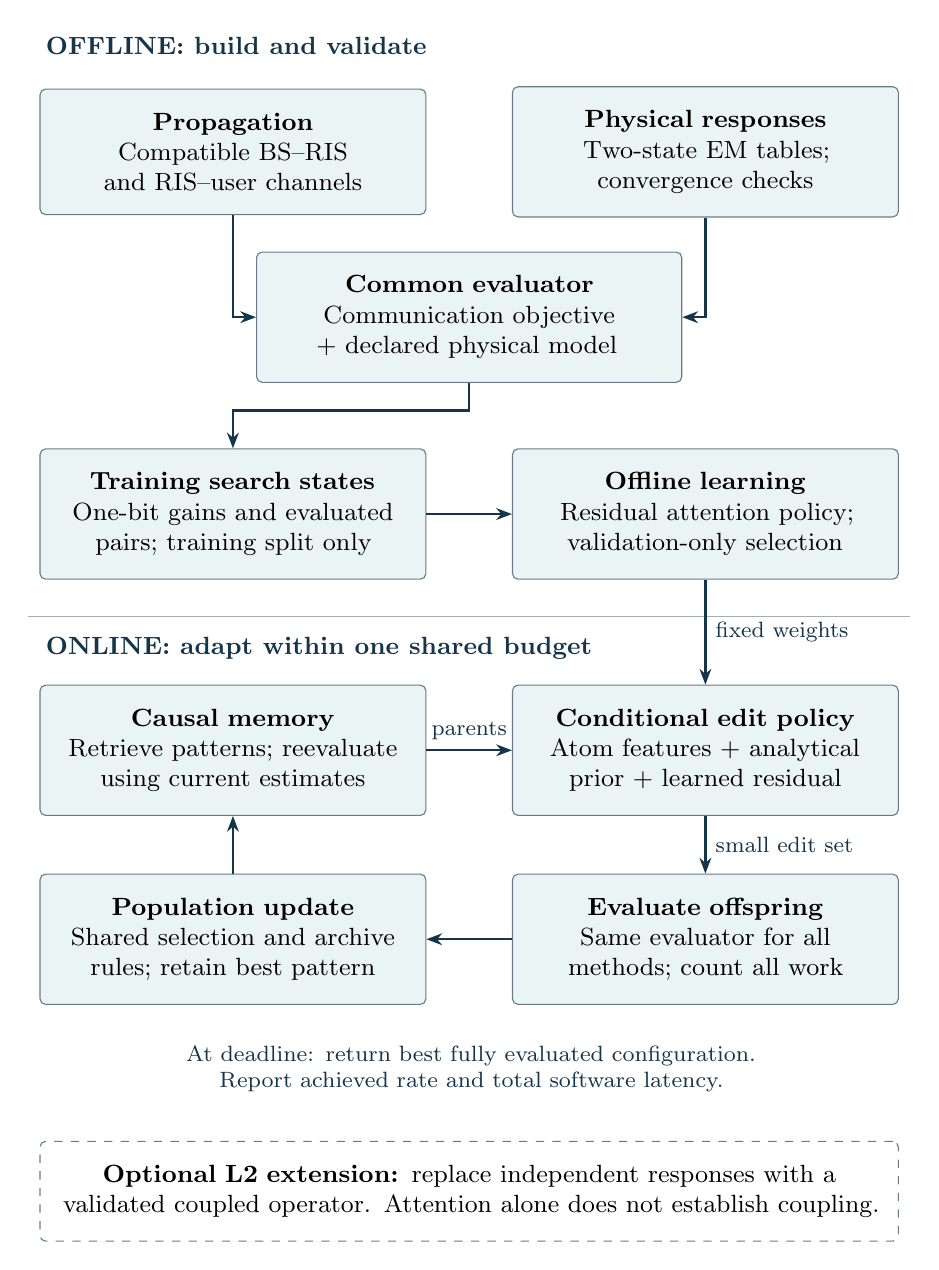
\begin{tikzpicture}[
  box/.style={draw=navy!65,rounded corners=2pt,fill=pale,align=center,font=\small,text width=43mm,minimum height=13mm,inner sep=3mm},
  flow/.style={-{Stealth[length=2mm]},thick,draw=navy},
  note/.style={font=\footnotesize,align=center,text=navy}
]
\node[box] (prop) at (0,0) {\textbf{Propagation}\\Compatible BS--RIS and RIS--user channels};
\node[box] (em) at (6.0,0) {\textbf{Physical responses}\\Two-state EM tables; convergence checks};
\node[note,anchor=west,font=\bfseries\small] at (-2.5,1.35) {OFFLINE: build and validate};
\node[box,text width=48mm] (eval) at (3,-2.1) {\textbf{Common evaluator}\\Communication objective + declared physical model};
\draw[flow] (prop.south) |- (eval.west);
\draw[flow] (em.south) |- (eval.east);
\node[box] (data) at (0,-4.6) {\textbf{Training search states}\\One-bit gains and evaluated pairs; training split only};
\node[box] (train) at (6,-4.6) {\textbf{Offline learning}\\Residual attention policy; validation-only selection};
\draw[flow] (eval.south) -- ++(0,-0.35) -| (data.north);
\draw[flow] (data) -- (train);
\draw[navy!40] (-2.6,-5.9) -- (8.6,-5.9);
\node[note,anchor=west,font=\bfseries\small] at (-2.5,-6.3) {ONLINE: adapt within one shared budget};
\node[box] (memory) at (0,-7.6) {\textbf{Causal memory}\\Retrieve patterns; reevaluate using current estimates};
\node[box] (policy) at (6,-7.6) {\textbf{Conditional edit policy}\\Atom features + analytical prior + learned residual};
\draw[flow] (train.south) -- node[right,note]{fixed weights} (policy.north);
\draw[flow] (memory) -- node[above,note]{parents} (policy);
\node[box] (update) at (0,-10.0) {\textbf{Population update}\\Shared selection and archive rules; retain best pattern};
\node[box] (score) at (6,-10.0) {\textbf{Evaluate offspring}\\Same evaluator for all methods; count all work};
\draw[flow] (policy) -- node[right,note]{small edit set} (score);
\draw[flow] (score) -- (update);
\draw[flow] (update) -- (memory);
\node[note,text width=105mm] at (3,-11.65) {At deadline: return best fully evaluated configuration.\\Report achieved rate and total software latency.};
\node[box,dashed,fill=white,text width=103mm,minimum height=9mm] at (3,-13.2) {\textbf{Optional L2 extension:} replace independent responses with a validated coupled operator. Attention alone does not establish coupling.};
\end{tikzpicture}

\caption{Proposed workflow; no measured performance is implied. Offline propagation and EM data produce a validated common evaluator and training trajectories. Online, physical features and search state guide conditional edits of remembered candidates. Solid arrows show the core L1 pipeline; the dashed block is a separately validated L2 extension. The loop returns the best evaluated configuration before its budget expires.}
\label{fig:framework}
\end{figure*}

\subsection{Atom tokens and attention}
For candidate $\bvec$, token $\mathbf x_n$ contains its current bit, real/imaginary parts of both physical responses and their contrast, normalized position, per-user/stream channel contribution summaries, analytical flip score, population bit frequency, and recent accepted-edit history. Global features include user rates, remaining budget, stagnation, and memory age. Features must be obtainable from the declared observation model. They exclude future channels and test-only clean CSI.

A shared encoder maps tokens to width $d=32$ or $64$. Two attention layers will be tested, with global summary tokens and a small spatial neighborhood. The neighborhood is an architectural prior, not evidence of physical coupling. Full attention and a shared MLP with the same global summaries are controls; long-range communication interactions can make purely local attention insufficient. Relative positions travel with their tokens so reindexing a surface does not change its physical description.

Let $\widetilde g_n$ be the normalized analytical flip score (L0/L1), or a labeled independent-element proxy (L2). The residual policy forms
\[
s_n=\beta\,\widetilde g_n+r_\theta(\mathbf x_n,\{\mathbf x_m\},\mathbf z),
\]
with $\beta$ selected on validation data. Physics guidance refers to explicit features and an analytical prior; it does not imply that attention solves Maxwell's equations or that the network uses a PDE residual loss.

\subsection{Conditional edit sampling}
A categorical distribution over eligible elements is
\[
q(n\mid\mathcal S)=
\frac{(1-\epsilon)\exp(s_n/\tau)}
{\sum_{m\notin\mathcal S}\exp(s_m/\tau)}
+\frac{\epsilon}{N-|\mathcal S|}.
\]
This applies to $n\notin\mathcal S$.
Here $\mathcal S$ is the set already selected for this offspring. This is an element-selection distribution, \emph{not} $N$ independent Bernoulli probabilities. Sample a mutation count $m$ from a fixed, validation-selected distribution on $\{1,2,4\}$, shared across matched location-policy ablations. Select $m$ distinct elements sequentially, updating the candidate and available analytical features after each provisional edit. Commit the offspring to population selection only after evaluating the completed edit set.

Sequential conditioning lets the second edit depend on the first, but incurs overhead. A nonconditional sampling ablation tests its value. The exploration floor $\epsilon>0$ and shared random immigrants prevent permanent exclusion of elements; they do not guarantee escape from every local optimum.

\subsection{Offline training with explicit supervision}
Training data include baseline search states, random states, perturbed elites, and later training-only policy rollouts. The last source reduces mismatch between teacher states and states visited by the learned controller.

For one-bit moves, collect true objective differences. For selected parents, enumerate all pairs when $N$ is small and sample a balanced mixture of uniform, adjacent, and high-score pairs at $N=64$. Evaluate completed pairs, including cases where the first flip is harmful but the pair is beneficial. Good search must not be equated with greedily selecting individually positive flips.

For a sampled action set $\mathcal A$, define $G(a)=F(\bvec\oplus a)-F(\bvec)$ and
\[
y(a)=\frac{\exp(G(a)/T)}{\sum_{a'\in\mathcal A}\exp(G(a')/T)}.
\]
Train using cross-entropy on these soft targets, with an auxiliary gain-regression loss if validation supports it. For pair $\{i,j\}$, its policy probability is
$q(i)q(j\mid i)+q(j)q(i\mid j)$; normalize over the sampled pair set for the loss. The teacher is exact only over the sampled actions, not globally optimal. Use separate one-bit and pair losses so the fixed mutation-count distribution is not inadvertently learned.

Mutation size four is initially an exploration option, not directly supervised by pair labels. Larger-edit training is conditional on demonstrated benefit. Online policy-gradient training is outside the core study. Record teacher evaluations, EM generation, training time, and memory costs separately from online inference.

\subsection{Memory and evolutionary integration}
Use one shared ME-GA adaptation with identical selection, crossover, elitism, mutation-count distribution, archive size, and random-immigrant rules. Only mutation-location scoring changes in the main comparison. Document departures from Zardi et al.'s setup and information assumptions \cite{zardi}; call it an adaptation unless an exact reproduction is demonstrated.

At a new snapshot, retrieve prior patterns using currently available context, reevaluate them, and seed part of the population. Old fitness values never substitute for current evaluations. Memory retrieval and maintenance consume online budget. Memory is causal and resets at every independent test trajectory.
\begin{enumerate}[label=\arabic*.]
\item Receive current estimates and response descriptors; start the timer.
\item Retrieve and reevaluate remembered candidates; initialize other members.
\item Select parents and apply shared crossover.
\item Extract features and sample conditional edits.
\item Evaluate offspring with the common objective; update population and archive.
\item Repeat within budget; return the best fully evaluated feasible pattern.
\end{enumerate}
When no new pattern can be evaluated in time, use the previously available configuration. Report cold-start initialization and the fallback's current rate explicitly.

\section{Experimental design}
\subsection{Splits and scenarios}
Split by complete trajectories and disjoint spatial regions before generating optimization labels. A nominal 60/20/20 train/validation/test allocation will be fixed after inspecting scenario coverage, with spatial buffers to reduce near-duplicate leakage. Never split adjacent samples from one trajectory across partitions. Use geometrically ordered positions for dynamics, not shuffled channels. If phase continuity is unsupported, call the experiment a sequence of quasi-static locations rather than a Doppler-valid mobile simulation.

Physical-response splits are separate. Interpolation tests hold out angle/frequency samples within a characterized family; transfer tests hold out complete load/geometry families. Frequency experiments regenerate compatible propagation data. Descriptor conditioning cannot establish design transfer when all splits use one unit cell. If only one design is feasible, narrow the claim to operating-condition transfer.

\begin{table}[t]
\caption{Planned benchmark tiers. Settings are design targets, not completed runs.}
\small
\begin{tabularx}{\linewidth}{@{}p{20mm}YY@{}}
\toprule
Tier & Configuration & Purpose\\
\midrule
Sanity & $N\in\{8,16\}$, $K=1,2$; L0/L1. & Exhaustive optimum and exact-flip verification.\\
Core static & $N=64$, $K=2,4$; L1. & Rate versus evaluation and time budgets.\\
Core sequential & Held-out trajectories; fixed update schedule. & Memory benefit and adaptation at deadlines.\\
Robustness & Held-out response conditions; CSI NMSE at $-30,-20,-10$ dB. & Sensitivity to estimated inputs and distribution shift.\\
Extension & L2 at validated sizes; optional $N=256$ L1. & Coupling and scaling without unsupported extrapolation.\\
\bottomrule
\end{tabularx}
\end{table}

The initial final-study target is at least 30 independent test trajectories and 10 paired optimizer seeds. A training/validation-only pilot estimates variance and determines whether more trajectories are required for stable effect estimates. Trajectory, not each correlated time step, is the principal statistical unit.

\subsection{Baselines that can falsify the proposal}
\begin{enumerate}
\item \textbf{Exact/specialized control:} exhaustive search at small $N$; applicable optimal binary single-user solver \cite{zhang} on compatible L0 models. Verify assumptions before extending it.
\item \textbf{Analytical local search:} vectorized exact-gain greedy flips with restarts; best-pair or sampled-pair search under equal time budgets. Use cached updates, not intentionally slow recomputation.
\item \textbf{Evolutionary control:} random search, conventional GA, adaptive GA, and the shared ME-GA adaptation.
\item \textbf{Physics-guided ME-GA:} sample locations from analytical scores without a network, using the same exploration and mutation-count rules.
\item \textbf{Learned controls:} capacity-matched shared MLP, attention without physical descriptors, and attention without conditional updates. All receive the same permitted global/search information.
\item \textbf{Direct prediction:} small one-pass binary predictor trained on the same partition, optionally followed by equal-budget local refinement. This tests whether iterative machinery is necessary.
\end{enumerate}
Matched mutation ablations use identical GA settings to isolate causality. A separate best-tuned comparison permits method-specific settings with equal validation tuning budgets. These answer different questions.

\subsection{Factorial ablations}
The minimum grid crosses memory on/off, physical descriptors on/off, and MLP/attention. Additional tests remove the analytical prior or conditional selection, and replace learned scores with exact-gain scores. Use the same evaluator and mutation-count distribution. Report parameters, operation counts where available, and measured latency; parameter count alone does not establish matched computational cost.

On L1, exact flip gains already contain physical information. Therefore test descriptor ablations both with and without those gains. Removing the raw response table while retaining its exact consequences is not a clean test of whether physics is useful.

\subsection{Budgets, endpoints, and statistics}
Two separate protocols will be used:
\begin{itemize}
\item \textbf{Evaluation-budget protocol:} equal counted evaluator work, including candidate and feature-scoring calls. Log analytical updates separately with their arithmetic/time cost rather than treating them as free oracle queries.
\item \textbf{Wall-clock protocol:} equal deadlines on the same CPU, fixed threads and precision, including retrieval, features, sampling, inference, scoring, and updates. GPU results, if included, are separate and include transfer/synchronization costs.
\end{itemize}
Candidate CPU deadlines are 1, 5, 10, 50, and 100 ms. Check feasibility on validation data and freeze the primary deadline before opening test results. These are computation benchmarks, not promised radio coherence times. At least one deadline must let all main methods return an evaluated configuration. Report median and 95th-percentile latency, initialization cost, model size, and peak memory. A100 access supports training; it does not establish low-power feasibility.

\textbf{Primary endpoint:} paired difference in mean trajectory worst-user rate between the proposed policy and the strongest validation-selected non-neural baseline at the frozen deadline. Also compare with matched ME-GA and MLP. Report absolute bit/s/Hz differences and relative changes with the denominator specified.

\textbf{Secondary endpoints:} rate-versus-budget curves, evaluated candidates, post-change adaptation loss, switch counts, and time to a prespecified target. A high-budget reference is called best found, not optimal, except where proven or exhaustive optimization applies. Fix the target rule before testing; count failures to reach it as censored observations.

Use paired trajectory-level bootstrap confidence intervals, keeping entire time series within resampled trajectories and aggregating seeds consistently. Prespecify one primary comparison and apply Holm correction to declared secondary tests. Report per-scenario and negative results, not just a favorable pooled mean.

For imperfect CSI, search uses estimates and model-derived fitness; final scoring uses clean held-out channels. This avoids falsely granting the controller clean feedback. Pilot overhead, RF switching latency, and energy are not measured by software timings and will not be claimed.

\section{Validation gates and risks}
\begin{table}[t]
\caption{Milestones that prevent an unsupported final claim.}
\small
\begin{tabularx}{\linewidth}{@{}p{19mm}YY@{}}
\toprule
Gate & Evidence required & Consequence if unmet\\
\midrule
G1: physics & Mesh convergence, extraction record, compatible normalization, and independent small-case checks. & Label synthetic-response results algorithmic, not EM-validated.\\
G2: relevance & Nonideal ranking changes or material rate loss under the common evaluator. & Narrow or abandon the response-awareness novelty claim.\\
G3: search & Gains over exact-score, pair-search, MLP, and memory controls. & Prefer the simpler method and report the negative result.\\
G4: runtime & Positive primary endpoint after neural overhead. & Claim evaluation efficiency only if supported, not a faster controller.\\
G5: coupling & Held-out full-wave agreement, optimized-pattern audits, and size-transfer evidence where needed. & Limit L2 to validated sizes or omit it.\\
\bottomrule
\end{tabularx}
\end{table}

For surrogate-based L2, report complex-field error, rate error, and ranking agreement on ordinary held-out and optimizer-selected patterns. Audit finalists from \emph{all} methods under the same high-fidelity budget. Distinguish numerical solver, surrogate, and channel-model error. A small average prediction error does not guarantee correct ranking near an optimum.

The main scientific risk is that analytical updates already solve adaptation adequately. This is a legitimate negative outcome. Other risks are expensive EM sweeps, incompatible geometry, memory overfitting to nearby locations, and attention overhead. Start small, retain strong baselines, and freeze the evaluation protocol before large training.

\section{Work plan, resources, and reproducibility}
\begin{table*}[t]
\caption{Nine-month core plan with a conditional extension.}
\small
\begin{tabularx}{\linewidth}{@{}p{19mm}YY@{}}
\toprule
Period & Work & Deliverable / decision\\
\midrule
Month 1 & Prior art, analytical checks, scenario/solver feasibility. & Final claim boundary and feasibility report.\\
Months 2--3 & Propagation interface, EM extraction, mesh checks. & Versioned L0/L1 evaluator; G1/G2 decisions.\\
Month 4 & Analytical, pair-search, GA, ME-GA; runtime profiling. & Baselines and frozen budget protocol.\\
Month 5 & Training trajectories; MLP and attention policies. & Trained candidates and offline-cost ledger.\\
Month 6 & Conditional edits, memory integration, model selection. & Frozen architecture and test plan.\\
Months 7--8 & Core tests, ablations, robustness, statistics. & G3/G4 decisions and complete results.\\
Month 9 & Error analysis, artifact audit, manuscript. & Core paper and reproducibility package.\\
Months 10--12 & Validated L2 or scaling study if core is stable. & G5 decision and separated extension.\\
\bottomrule
\end{tabularx}
\end{table*}

Use existing institutional CPU/GPU resources. GPUs support offline learning; EM feasibility depends on CPU memory and solver support, which A100 access does not eliminate. No RIS fabrication, RF equipment, IoT board, or new software license is required by the core plan. Estimate storage and compute hours from a small pilot before broad generation. Publication fees, electricity, institutional resource costs, and researcher time are separate from a zero-purchase budget.

Release scripts, manifests, split identifiers, response provenance, solver versions, hashes, seeds, checkpoints, environments, and per-run traces where licenses permit. Keep immutable test partitions and a validation-decision log. Every plot should be reproducible from saved results. Store actual rates, failures, and timing distributions; projected values are not results.

\section{Expected significance and claim boundaries}
The strongest outcome is a reproducible demonstration that response-conditioned learning selects useful groups of edits that analytical local search misses under the same deadline. This would connect element-level physics to adaptive search behavior, with evidence surviving memory and architecture controls.

A weaker but informative outcome is a measured boundary: independent elements, small arrays, or tight deadlines may favor analytical methods; learning may help only with more demanding objectives or validated interactions. The study will not claim first-ever physics-aware RIS optimization, global optimality, full-array coupling from unit-cell data alone, measured hardware gains, or real-time MCU deployment.

\begin{thebibliography}{12}
\bibitem{zhang} Y. Zhang, K. Shen, S. Ren, X. Li, X. Chen, and Z.-Q. Luo, ``Configuring Intelligent Reflecting Surface with Performance Guarantees: Optimal Beamforming,'' \emph{IEEE Journal of Selected Topics in Signal Processing}, 2022. \href{https://doi.org/10.1109/JSTSP.2022.3176479}{doi:10.1109/JSTSP.2022.3176479}. Author preprint: \url{https://arxiv.org/abs/2112.02260}.
\bibitem{zardi} F. Zardi, G. Oliveri, and A. Massa, ``Memory-Enhanced Dynamic Evolutionary Control of Reconfigurable Intelligent Surfaces,'' \emph{IEEE Transactions on Antennas and Propagation}, vol. 72, no. 7, pp. 5754--5766, 2024. \href{https://doi.org/10.1109/TAP.2024.3407964}{doi:10.1109/TAP.2024.3407964}.
\bibitem{lange} R. T. Lange, T. Schaul, Y. Chen, C. Lu, T. Zahavy, V. Dalibard, and S. Flennerhag, ``Discovering Attention-Based Genetic Algorithms via Meta-Black-Box Optimization,'' \emph{GECCO}, 2023. \href{https://doi.org/10.1145/3583131.3590496}{doi:10.1145/3583131.3590496}. Author preprint: \url{https://arxiv.org/abs/2304.03995}.
\bibitem{qian} X. Qian and M. Di Renzo, ``Mutual Coupling and Unit Cell Aware Optimization for Reconfigurable Intelligent Surfaces,'' arXiv preprint, 2020. \url{https://arxiv.org/abs/2011.14373}.
\bibitem{risnet} B. Peng, K.-L. Besser, S. Shen, F. Siegismund-Poschmann, R. Raghunath, D. Mittleman, V. Jamali, and E. A. Jorswieck, ``RISnet: A Domain-Knowledge Driven Neural Network Architecture for RIS Optimization with Mutual Coupling and Partial CSI,'' arXiv preprint, 2024. \url{https://arxiv.org/abs/2403.04028}.
\bibitem{liu} W. Liu, W. Chen, C. Chen, X. Zhang, and S. An, ``Physics Informed Generative Surrogate Learning for Full Wave Validated Real Time Beamforming in Programmable Metasurfaces,'' \emph{Advanced Electronic Materials}, e70480, 2026. \href{https://doi.org/10.1002/aelm.70480}{doi:10.1002/aelm.70480}.
\bibitem{urbinati} L. Urbinati, N. Decarli, F. Guidi, A. Guerra, B. M. Masini, and A. Zanella, ``On-Device Deep Learning for RIS Beamforming: Design and Latency-Rate Trade-Offs,'' \emph{IEEE Open Journal of the Communications Society}, vol. 7, pp. 4605--4622, 2026. \href{https://doi.org/10.1109/OJCOMS.2026.3687306}{doi:10.1109/OJCOMS.2026.3687306}.
\bibitem{martin} A. Mart\'in-Mart\'in, R. Padial-Allu\'e, E. Castillo, L. Parrilla, I. Parellada-Serrano, A. Mor\'an, and A. Garc\'ia, ``Hardware Implementations of a Deep Learning Approach to Optimal Configuration of Reconfigurable Intelligence Surfaces,'' \emph{Sensors}, vol. 24, no. 3, 899, 2024. \href{https://doi.org/10.3390/s24030899}{doi:10.3390/s24030899}.
\bibitem{zheng} P. Zheng, R. Wang, A. Shamim, and T. Y. Al-Naffouri, ``Mutual Coupling in RIS-Aided Communication: Model Training and Experimental Validation,'' arXiv preprint, 2023; revised 2024. \url{https://arxiv.org/abs/2311.10544}.
\bibitem{deepmimo} DeepMIMO contributors, ``DeepMIMO documentation and channel generator,'' official software repository and manual. Accessed 21 October 2026. \url{https://github.com/DeepMIMO/DeepMIMO}; \url{https://www.deepmimo.net/docs/tutorials/manual.html}.
\bibitem{openems} T. Liebig and openEMS contributors, ``openEMS: Open-source electromagnetic field solver,'' official source repository. Accessed 21 October 2026. \url{https://github.com/thliebig/openEMS}.
\bibitem{openemsbc} openEMS contributors, ``FDTD Boundary Conditions,'' official project documentation. Accessed 21 October 2026. \url{https://wiki.openems.de/index.php/FDTD_Boundary_Conditions.html}.
\end{thebibliography}

\end{document}
